\documentclass{article}
\usepackage{tikz, comment}
\usepackage{pifont}
\usepackage{fontspec}
\usetikzlibrary{arrows, decorations.markings, decorations.pathreplacing}
\begin{comment}
:Title: Not defined yet
:Slug: No name yet

Description Here.........
\end{comment}
\begin{document}\centering 

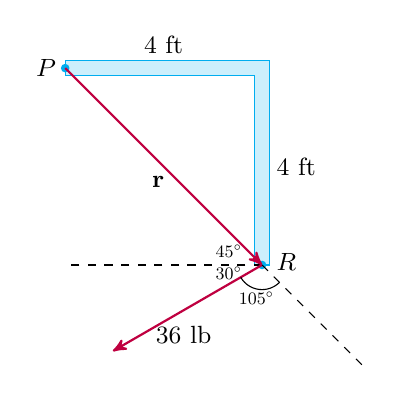
\begin{tikzpicture}[>=latex,xscale=.5*1.25, yscale=.5*1.25][font=\sf\small] 

\draw[cyan, fill=cyan!20] (0, 0)--++(-0.15, 0)--++(0, {4-0.15})--++({-4+0.15}, 0)--++(0, {0.15*2})--++({4+0.15}, 0)--++(0, {-4-0.15})--++(-0.15, 0);

\draw[cyan, fill] (-4,4) circle(0.075)node[black, left] {$P$};

\draw[cyan, fill] (0,0) circle(0.075)node[black, right, xshift=2, yshift=1]{$R$};

\node[above, yshift=2] at (-2, 4) {\rm $4$ ft};
\node[right, xshift=2] at (0, 2) {\rm $4$ ft};

\draw[dashed] (0,0)--++(-4, 0); 

\draw[purple, thick, ->, >=stealth'] (-4, 4)--(0,0)
node[black, below, midway, pos=0.5, xshift=-2, yshift=0, scale=1]{${\bf r}$};;

\draw[purple, thick, ->, >=stealth'] (0,0)--({3.5*cos(-150)}, {3.5*sin(-150)})
node[black, below, midway, pos=0.6, xshift=4, yshift=0, scale=1]{\rm $36$ lb};;

\draw[dashed] (0,0)--({3*cos(-45)}, {3*sin(-45)});

\draw[samples=100, smooth, domain=-45:-150, variable=\x] 
		plot ({0.5*cos(\x)}, {0.5*sin(\x)}); 
\node[xshift=-2, yshift=-12, scale=0.7] at (0,0) {$105^\circ$};		

\node[xshift=-12, yshift=-3, scale=0.7] at (0,0) {$30^\circ$};	
\node[xshift=-12, yshift=5, scale=0.7] at (0,0) {$45^\circ$};	

\end{tikzpicture}
\end{document}